\documentclass[tikz,border=4pt]{standalone}
\usepackage[T1]{fontenc}
\usepackage[utf8]{inputenc}
\usepackage{amsmath,amssymb}
\usepackage{helvet}
\renewcommand{\familydefault}{\sfdefault}
\usepackage{pgfplots}
\pgfplotsset{compat=1.17}
\usetikzlibrary{arrows.meta,positioning,calc,fit,backgrounds,shapes.geometric}

\definecolor{cVis}{HTML}{1F77B4}
\definecolor{cTxt}{HTML}{D62728}
\definecolor{cProj}{HTML}{2CA02C}
\definecolor{cLLM}{HTML}{9467BD}
\definecolor{cConv}{HTML}{FF7F0E}
\definecolor{cAtt}{HTML}{17BECF}
\definecolor{cGray}{HTML}{7F7F7F}

\tikzset{
  blk/.style={draw, rounded corners=2pt, minimum height=8mm, align=center, font=\footnotesize, thick},
  tok/.style={draw, minimum size=3.2mm, inner sep=0pt},
  arr/.style={-{Stealth[length=2mm]}, thick},
}

\begin{document}
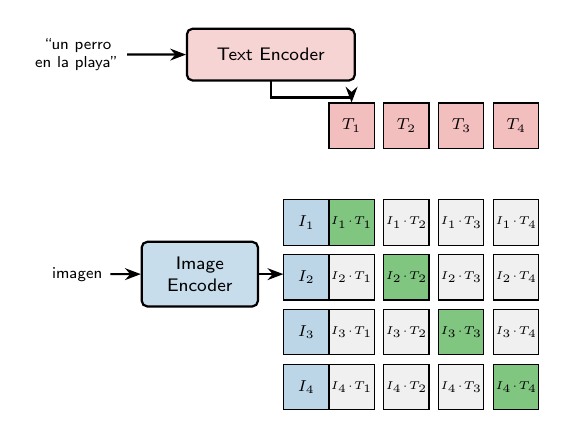
\begin{tikzpicture}[scale=.82, every node/.style={transform shape}]
  \node[blk, fill=cTxt!20, minimum width=26mm] (te) at (0,4.2) {Text Encoder};
  \node[font=\scriptsize, align=center] (tx) at (-3.0,4.2) {``un perro\\en la playa''};
  \draw[arr] (tx) -- (te);
  \foreach \j in {1,...,4}{\node[tok,fill=cTxt!30,minimum size=7mm] (T\j) at (0.4+\j*0.85,3.1) {\scriptsize$T_\j$};}
  \draw[arr] (te.south) -- ++(0,-0.25) -| (T1.north);
  \node[blk, fill=cVis!25, minimum width=18mm, minimum height=10mm] (ie) at (-1.1,0.8) {Image\\Encoder};
  \node[font=\scriptsize] (ix) at (-3.0,0.8) {imagen};
  \draw[arr] (ix) -- (ie);
  \foreach \i in {1,...,4}{\node[tok,fill=cVis!30,minimum size=7mm] (I\i) at (0.55,2.45-\i*0.85) {\scriptsize$I_\i$};}
  \draw[arr] (ie.east) -- (I1.west |- ie.east);
  \foreach \i in {1,...,4}{\foreach \j in {1,...,4}{
    \ifnum\i=\j \def\cc{cProj!60}\else \def\cc{black!6}\fi
    \node[tok,fill=\cc,minimum size=7mm] at (0.4+\j*0.85,2.45-\i*0.85) {\tiny$I_\i\!\cdot\! T_\j$};}}
\end{tikzpicture}
\end{document}
